% Teto: 3.000 palavras no total (abertura: 100; 3.1: 500; 3.2: 250; 3.3: 650; 3.4: 200;
% 3.5: 900; 3.6: 400). Fonte: seção 3 do .docx (PR 55) e do esqueleto.
\section{Metodologia}

\pendente{abertura: o que mudou em relação ao TCC I}

\subsection{Captura e extração de features}

\pendente{3.1}

\subsection{Pré-processamento e amostragem}

\pendente{3.2}

\subsection{Treino e avaliação do classificador}

\pendente{3.3, com a regra de alarme decidida e a janela lenta não julgada (PR 61)}

\subsection{Justificativa do Random Forest}

\pendente{3.4, com a comparação com o benchmark dos autores do dataset (PR 59)}

\subsection{Servidor MCP e sistema multiagente}

\pendente{3.5: servidor, agentes, skills escritas pela equipe (tarefa 96), modelo local
(OBLITERATUS/Qwen3.8-27B-OBLITERATED, tarefa 91) e por que não o Jev (tarefa 94), uma frase
cada}

\begin{figure}[htb]
	\centering
	\caption{\pendente{legenda da arquitetura}}
	\label{fig:arquitetura}
	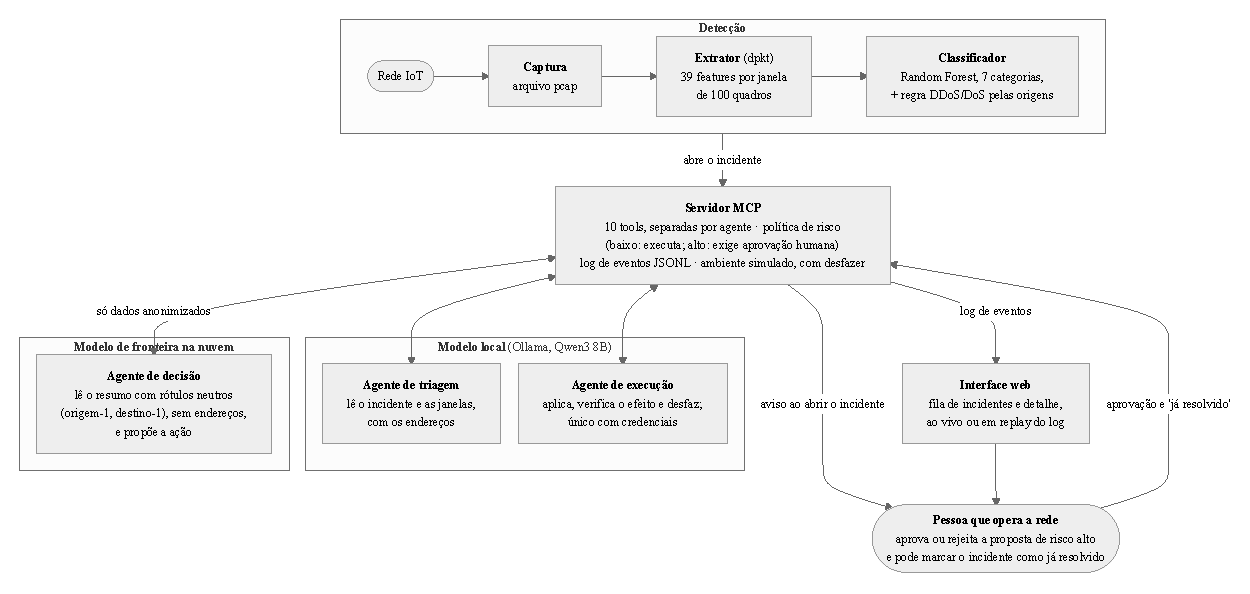
\includegraphics[width=\textwidth]{arquitetura.pdf}
	\legend{Fonte: os autores.}
\end{figure}

\begin{figure}[htb]
	\centering
	\caption{\pendente{legenda do fluxo de um incidente}}
	\label{fig:fluxo}
	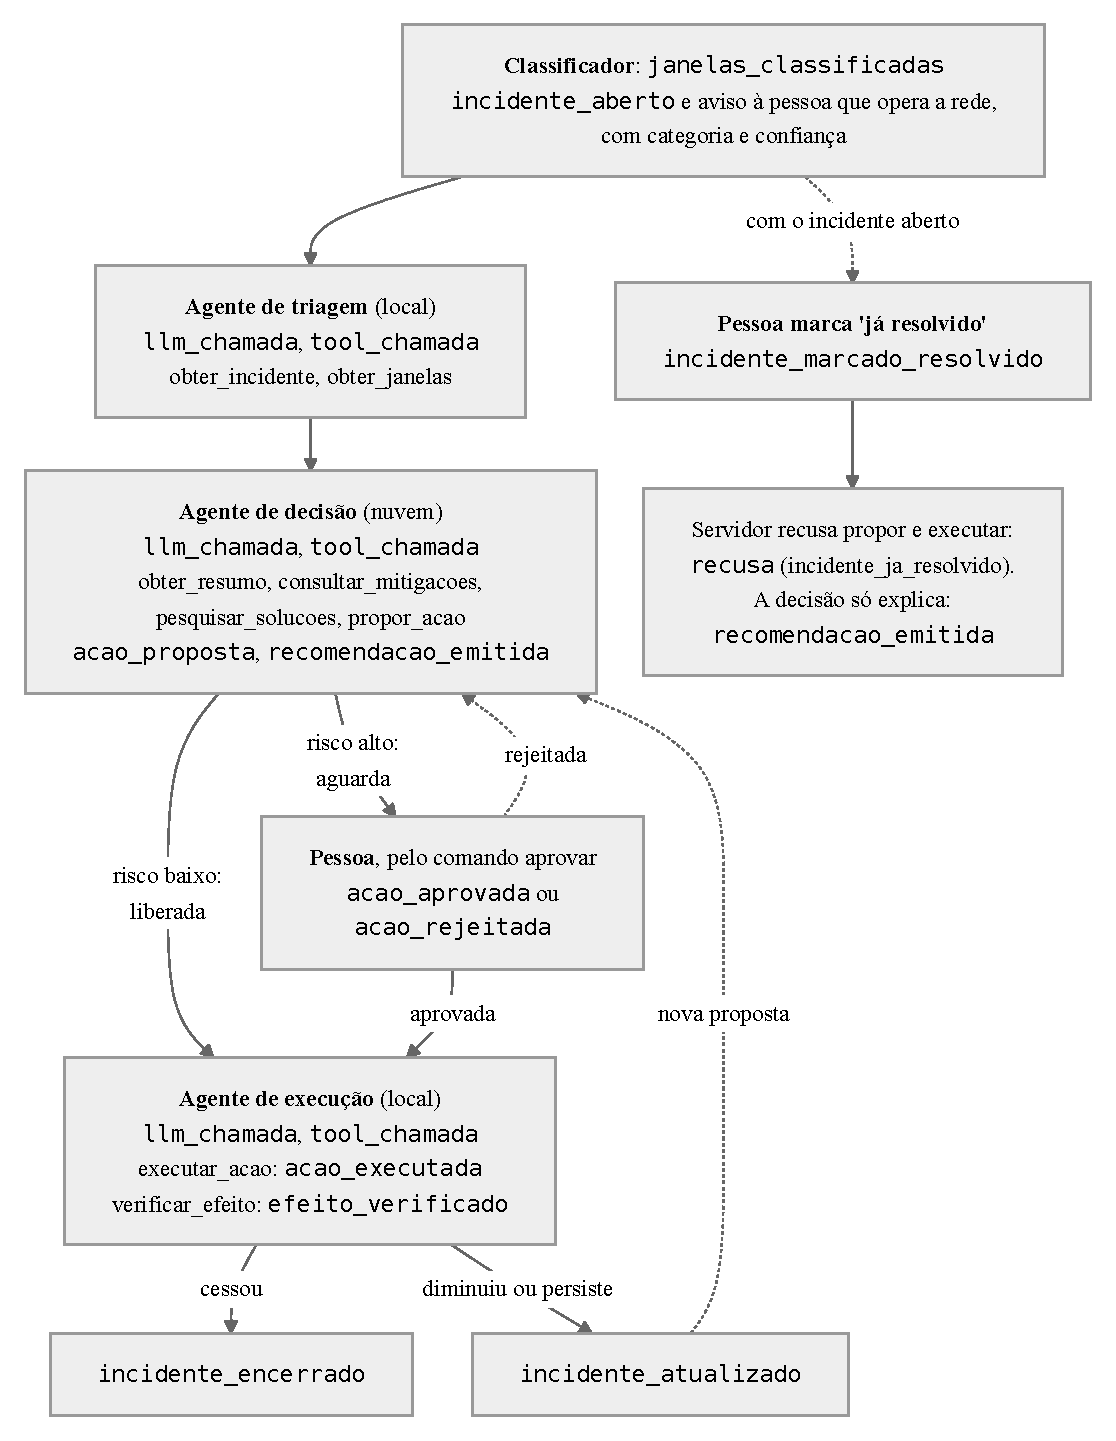
\includegraphics[width=\textwidth]{fluxo_incidente.pdf}
	\legend{Fonte: os autores.}
\end{figure}

\subsection{Avaliação da PoC e dos agentes}

\pendente{3.6, com o método do teste na casa (tarefa 93) e nos datasets externos (tarefa 95)}
